\documentclass[language=german,style=solution]{smo}

\title{Vorrunde 2019 - Musterlösung}

\begin{document}

\begin{enumerate}

\item[\textbf{G1)}]
Sei $k$ ein Kreis mit Mittelpunkt $O$ und seien $A$, $B$ und $C$ drei Punkte auf $k$ mit $\angle ABC > 90^\circ$. Die Winkelhalbierende von $\angle AOB$ schneide den Umkreis des Dreiecks $BOC$ ein zweites Mal in $D$. Zeige, dass $D$ auf der Geraden $AC$ liegt.

\textbf{Lösung (David):}
\begin{center}
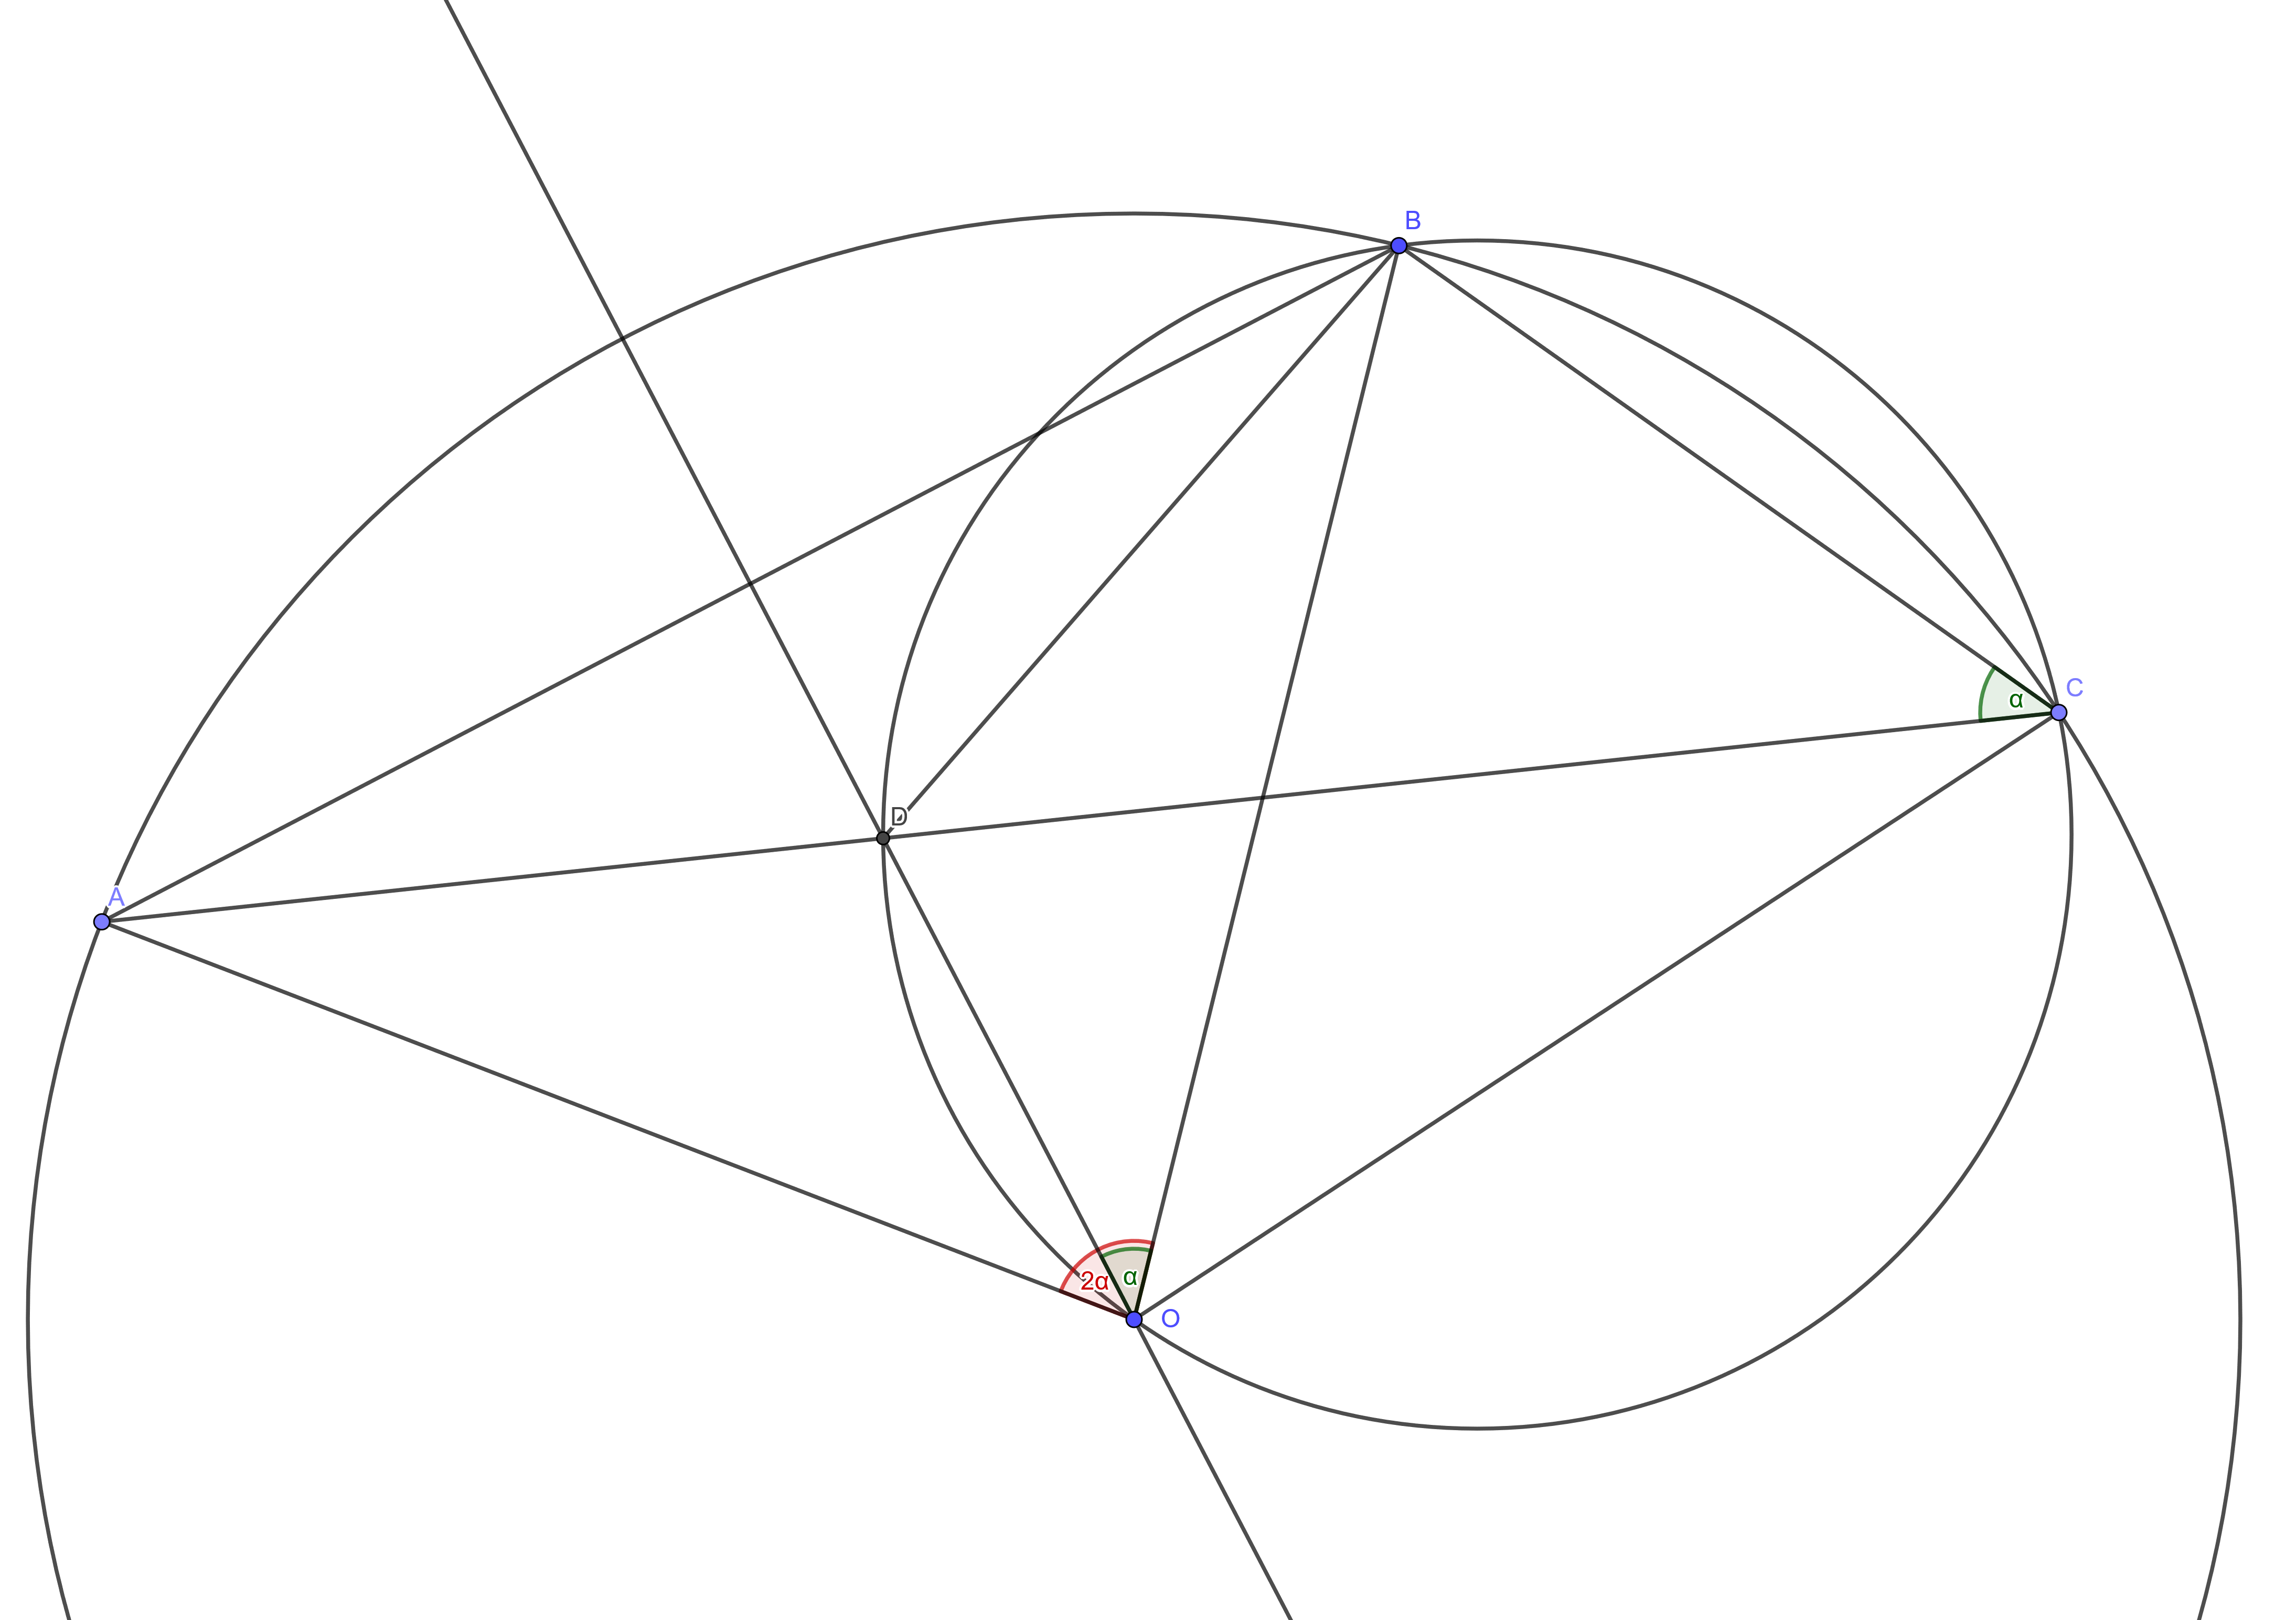
\includegraphics[width=0.8\textwidth]{Vorrunde_2019_G1.png}
\end{center}
\vspace{1cm}
Sei $\angle ACB = \alpha$. Wir wollen zeigen, dass auch $\angle DCB = \alpha$ gilt, dann liegen $A$, $D$ und $C$ auf einer Geraden.

Aufgrund des Zentriwinkelsatzes über der Sehne $AB$ gilt $\angle AOB = 2 \angle ACB = 2 \alpha$. Weil $OD$ die Winkelhalbierende des Winkels $\angle AOB$ ist, gilt somit $\angle DOB = \frac{1}{2} \angle AOB = \alpha$. 

Der Peripheriewinkelsatz über der Sehne $BD$ liefert nun $\angle DOB = \angle DCB$, also $\angle DCB = \alpha$, wie gewünscht.

\textbf{Marking Scheme}
\begin{itemize}
\item +1P: Idee, $\angle ACB = \angle DCB$ zu zeigen.
\item +2P: $\angle AOB = 2 \angle ACB$.
\item +1P: $\angle DOB = \angle ACB$.
\item +1P: $\angle DOB = \angle DCB$.
\item +2P: Fertig machen.
\end{itemize}
Maximal 1P für Winkel auf Skizzen ohne Begründung.

\newpage

\item[\textbf{G2)}]
Sei $k_1$ ein Kreis und $l$ eine Gerade, die $k_1$ in zwei verschiedenen Punkten $A$ und $B$ schneidet. Sei $k_2$ ein weiterer Kreis ausserhalb von $k_1$, der $k_1$ in $C$ und $l$ in $D$ berührt. Sei $T$ der zweite Schnittpunkt von $k_1$ und der Geraden $CD$. Zeige, dass $AT=TB$ gilt.

\textbf{1. Lösung (Paul):}\\
Um $AT=BT$ zu zeigen reicht es, die Winkelgleichung $\angle ABT = \angle TAB$ zu beweisen.\\
Sei $t$ die Tangente an $k_1$ in $C$ und $S$ der Schnittpunkt von $t$ und $l$. Dann ist $t$ auch die Tangente an $k_2$ in $C$, da die Kreise sich berühren. Sei $\beta = \angle SCB$ und $\alpha = \angle DCS$. Sei $E$ ein Punkt auf dem Kreis $k_2$ wie in der Skizze. Durch zweimaliges Anwenden des Tangentenwinkelsatzes erhält man $\angle SDC = \angle DEC = \angle DCS = \alpha$. Nun wenden wir nochmal den Tangentenwinkelsatz mit dem Dreieck $BCT$ und der Tangente $t$ an: $\angle CTB = \angle SCB = \beta$. Mit dem Aussenwinkelsatz im Dreieck $BDT$ gilt nun $\angle ABT = \angle BDT + \angle DTB = \alpha + \beta$. \\
Nun müssen wir noch $\angle TAB = \alpha + \beta$ zeigen.  Zuerst gilt $\angle BCT = 180-\angle DCB = 180 - \alpha - \beta$. Da $BCTA$ ein Sehnenviereck ist und die Winkel bei $A$ und $C$ sich gegenüberliegen, erhalten wir das Gewünschte.

\begin{center}
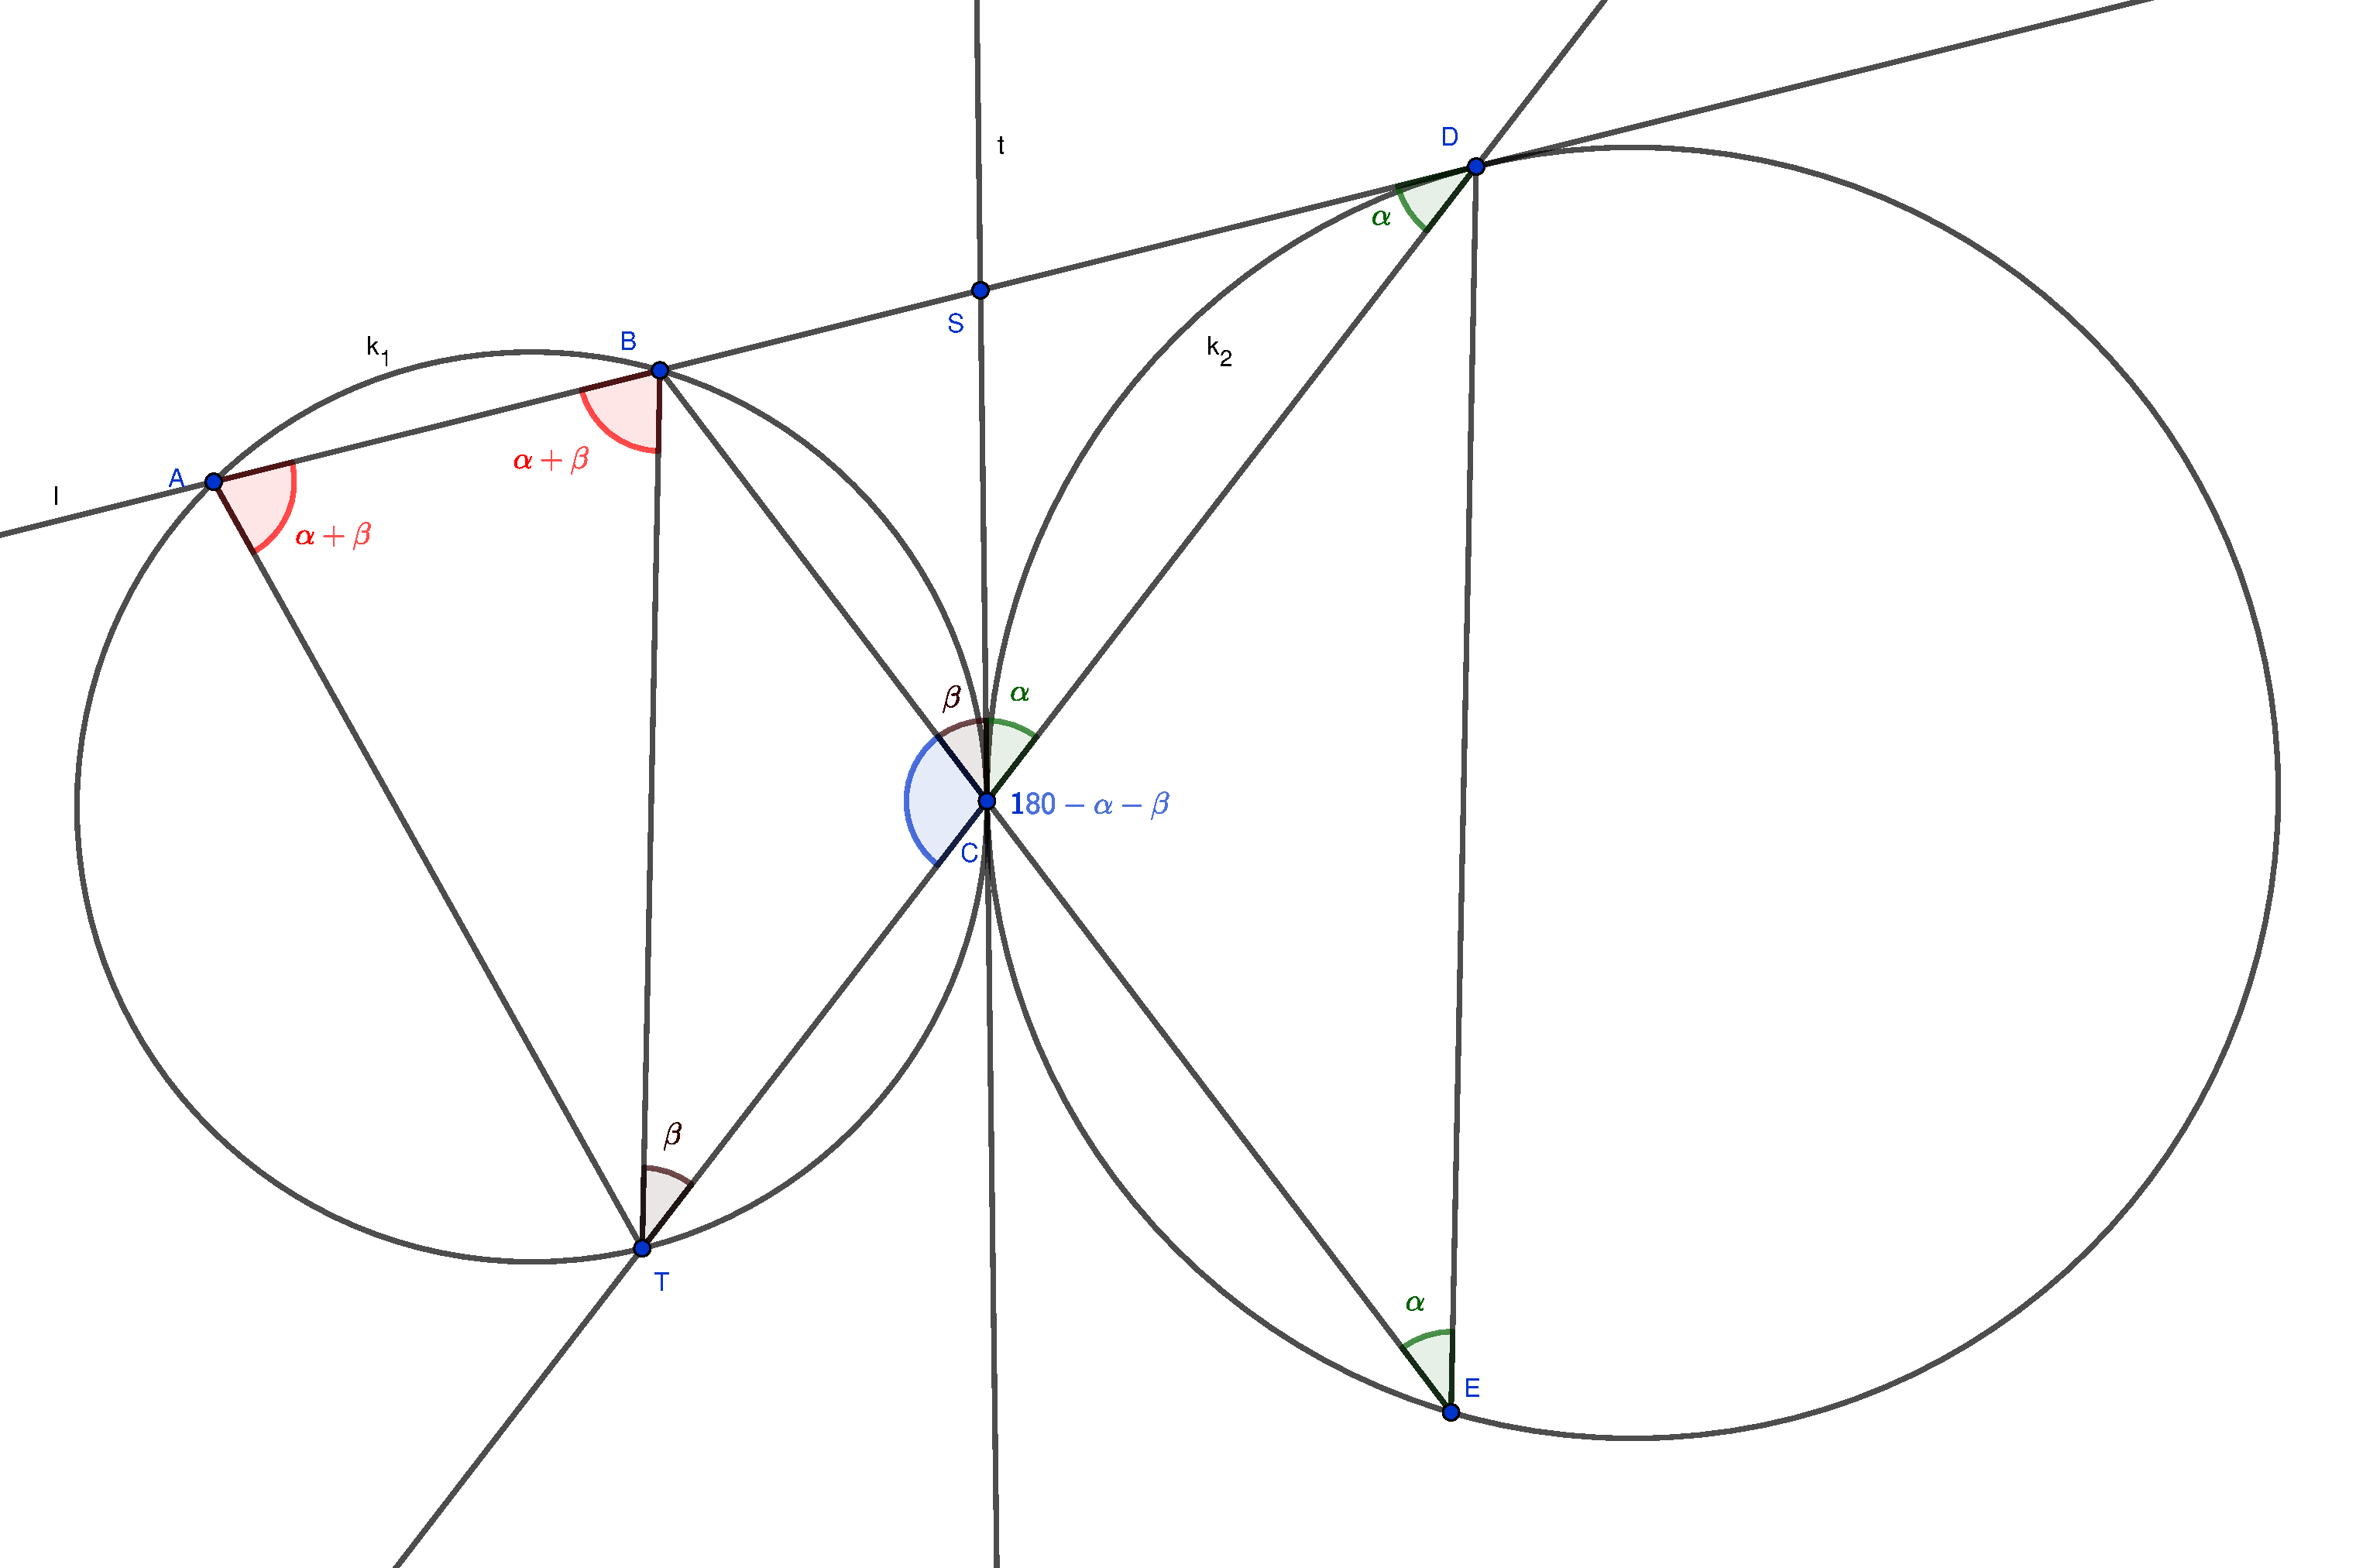
\includegraphics[width=0.8\textwidth]{muloe_G2.pdf}
\end{center}

\textbf{2. Lösung (Arnaud):}

Au lieu d'utiliser la condition de tangence des cercles en introduisant la tangente commune en $C$, on va utiliser l'homothétie. En effet, si l'on effectue une homothétie de centre $C$ et de rapport $-r_1/r_2$, où $r_i$ est le rayon du cercle $k_i$, alors on envoie $k_1$ sur $k_2$.

Comme l'homothétie préserve les droites qui passent par $C$ et comme $k_1$ est envoyé sur $k_2$, alors $T$ est envoyé sur $D$. De même, si l'on introduit $E$ la deuxième intersection de la droite $BC$ avec $k_2$, alors on remarque que l'homothétie envoie $B$ sur $E$. Une autre propriété fondamentale des homothéties implique que la droite $BT$ est envoyé sur une droite parallèle. Or l'image de $BT$ est précisément $ED$. On conclut donc que $BT$ est parallèle à $ED$.

Il ne reste plus que la chasse aux angles. Comme expliqué dans la première solution, on veut montrer que $\angle ABT=\angle TAB$. Comme les points $ABCT$ sont cocycliques, on obtient $\angle TAB=\angle 180^\circ -\angle TCB=\angle BCD$. De plus, comme $BD$ est tangente à $k_2$, le théorème de l'angle tangent nous donne $\angle CED=\angle CDB$. Comme les droites $TB$ et $ED$ sont parallèles, on obtient encore $\angle TBC=\angle CED$ et donc $\angle TBC=\angle CDB$. Au final, on a bien
\begin{align*}
\angle TBA&=180^\circ -\angle TBC-\angle CBD\\
&=180^\circ -\angle CDB-(180^\circ -\angle BCD-\angle CDB)\\
&= \angle BCD\\
&=\angle TAB.
\end{align*}

\textbf{3. Lösung (Arnaud):}

Cette fois-ci, on utilise la condition de tangence des cercles en introduisant les centres des deux cercles. Soit $O_1$ le centre de $k_1$ et $O_2$ le centre de $k_2$. Les deux cercles étant tangents en $C$, les points $O_1$, $O_2$ et $C$ sont alignés. Comme dans les autres preuves, on va montrer que $\angle TAB=\angle TBA$.

Soit $\alpha:=\angle ADT=\angle BDC$. Par le théorème de l'angle au centre couplé avec le théorème de l'angle tangent, on obtient $\angle DO_2C=2\alpha$. Le triangle $DO_2C$ est isocèle en $O_2$, donc $\angle O_2CD=\angle O_2DC=90^\circ -\alpha$. En utilisant, que $O_1,O_2$ et $C$ sont alignés, on obtient $\angle O_1CT=\angle O_2CD=90^\circ-\alpha$.

Soit $\beta:=\angle DTB$. Par le théorème de l'angle au centre $\angle CO_1B=2\beta$ et à nouveau on conclut que $\angle O_1CB=90^\circ-\beta$. On a ainsi $\angle TCB=\angle TCO_1+\angle O_1CB=180^\circ-\alpha-\beta$. Les points $ABCT$ étant cocycliques, on obtient $\angle TAB=180^\circ-\angle TCB=\alpha+\beta$.

De même, on a $\angle TBA=180^\circ -\angle TBD=180^\circ-(180^\circ-\angle BDT-\angle BTD)=\alpha+\beta$. Ce qui conclut la preuve.

\textbf{Marking Scheme - 1. Lösung:}
\begin{itemize}
    \item +1P: $\angle TAB = \angle DCB$.
    \item +1P: Die Tangente $t$ einführen und bemerken, dass sie an beiden Kreise tangent liegt.
    \item +1P: $\angle DCS = \angle SDC$.
    \item +1P: $\angle SCB = \angle CTB$. (1$\times$ Tangentenwinkelsatz)
    \item +1P: Wenn man beide Gleichungen hat.
    \item +1P: $\angle ABT = \angle DCB$.
    \item +1P: $\angle ABT = \angle TAB$ und begründen warum man dann fertig ist.
\end{itemize}

\textbf{Marking Scheme - 2. Lösung}:
    \begin{itemize}
        \item +1P: Spot the homothety with center $C$ between the two circles. 
        \item +1P: Introduce $E$ and use homothety to get $\angle TBE=\angle BED$.
        \item +1P: Using tangent angle $\angle CED=\angle CDB$.
        \item +1P: Both previous equalities. 
        \item +1P: Get $\angle TCB=\angle TBD.$
        \item +1P: $\angle ABT = \angle TAB$.
        \item +1P: Conclude.
    \end{itemize}
    
    \newpage
\textbf{Marking Scheme - 3. Lösung}:
    \begin{itemize}
        \item +1P: Introduce centers of the two circles and collinear with $C$.
        \item +1P: $\angle DO_2C=2\angle CDB$ (use the tangent and center).
        \item +1P: $\angle DO_2C=\angle TO_1C$ (use $C\in O_1O_2$).
        \item +1P: $2\angle TAC=\angle TO_1C$ (use center).
        \item +1P: $\angle BTC=\angle BAC$ (use Peripheriewinkelsatz).
        \item +1P: $\angle ABT = \angle TAB$.
        \item +1P: Conclude.
    \end{itemize}

\newpage

\item[\textbf{K1)}] 
Soit $n$ un entier strictement positif. Maurice écrit sur une même ligne tous les $2^n-1$ sous-ensembles non-vides de l'ensemble $\{1,2, \ldots, n \}$. Ensuite, en-dessous de chaque sous-ensemble, il écrit le produit de ses éléments. Finalement, il écrit les inverses des nombres présents sur la deuxième ligne et il en calcule la somme. Quelle sera la valeur de la somme (en fonction de $n$) que Maurice va obtenir ?

\emph{Exemple: pour $n=3$, Maurice obtient \vspace{-5mm} % <- don't know why this has to be here, probably for the same reason as above 
\begin{center}
\begin{tabular}{c c c c c c c c c c c c c c}
$\{1\}$ && $\{2\}$ && $\{3\}$ && $\{1,2\}$ && $\{1,3\}$ && $\{2,3\}$ && $\{1,2,3\}$&\\[1mm]
$1$ && $2$ && $3$ && $1 \cdot 2 = 2$ && $1\cdot 3 = 3$ && $2\cdot 3 = 6$ && $1\cdot 2 \cdot 3 = 6$&\\[1mm]
\Large$\frac{1}{1}$ &$+$& \Large$\frac{1}{2}$ & $+$ & \Large$\frac{1}{3}$ & $+$ &\Large$\frac{1}{2}$ & $+$ & \Large$\frac{1}{3}$ & $+$ & \Large$\frac{1}{6}$ &$+$& \Large$\frac{1}{6}$& \large $= 3.$\\
\end{tabular}
\end{center}
}%end emph


\textbf{1. Lösung (Louis):}

On commence par tester les petites valeurs de $n$ et on constate que à chaque fois la valeur obtenue est $n$. On pose donc l'hypothèse \[H(n) : \mbox{ La somme obtenue avec l'ensemble } \{1, 2, \ldots, n\} \mbox{ vaut } n\]
et on va essayer de prouver par induction que $H(n)$ est vérifiée pour tout nombre naturel $n$.

On commence par le cas de base $n=1$. Le seul sous-ensemble non-vide de $\{1\}$ est $\{1\}$, et le produit de ses éléments vaut $1$. Ainsi, la somme recherchée prend la valeur $1$ et le cas de base est démontré.

Pour le pas d'induction maintenant, supposons que $H(n)$ soit vérifiée et prouvons $H(n+1)$. On sépare les sous-ensembles non-vides en deux groupes. Le premier est constitué de tous les sous-ensembles qui ne contiennent pas $n+1$, et le second de tous les sous-ensembles qui contiennent $n+1$. Pour le premier groupe $H(n)$ prouve que la somme restreinte à ce groupe donne $n$. \newline
On veut donc prouver que pour le second groupe la somme restreinte à ce groupe vaut $1$. En retirant l'élément $n+1$ de chacun des sous-ensembles du deuxième groupe, on obtient tous les sous-ensembles de $\{1, 2, \ldots, n\}$ exactement une fois. En rajoutant $n+1$ à un sous-ensemble non-vide de $\{1, 2, \ldots, n\}$ on multiplie le produit de ses éléments par $n+1$. Puisqu'on prend ensuite l'inverse on divise donc la somme par $n+1$. En utilisant de nouveau $H(n)$ on voit qu'il faut donc encore rajouter $\frac{n}{n+1}$. Damnation! On voulait obtenir $1$, et on obtient à la place $\frac{n}{n+1}$. Est-ce que notre hypothèse est en fait fausse? Il s'avère qu'elle est correcte, et la différence vient du fait qu'on n'a pas encore considéré l'ensemble $\{n+1\}$, qui rajoute $\frac{1}{n+1}$ à la somme et prouve ainsi $H(n+1)$. Le problème est que ce sous-ensemble appartient clairement au deuxième groupe, mais en enlevant l'élément $n+1$ on obtient l'ensemble vide, donc vu que la somme dans $H(n)$ porte sur les sous-ensembles non-vides il ne faut pas oublier de rajouter encore la contribution provenant de ce sous-ensemble.

Comme le cas de base et le pas d'induction ont tous les deux été démontrés, le principe d'induction nous assure que $H(n)$ est satisfaite pour tous les entiers $n$, et donc la valeur obtenue avec cette somme est $n$.


\textbf{2. Lösung (Euler):}

La somme recherchée peut être réécrite sous la forme
\[
\prod_{i=1}^n\left(1+\frac{1}{i}\right)-1=\prod_{i=1}^n\left(\frac{i+1}{i}\right)-1=\frac{n+1}{1}-1=n.
\]

Observer que l'on soustrait 1 au produit parce que l'ensemble vide est exclu dans l'énoncé du problème.

\textbf{Marking Scheme - Première solution:}
	\begin{itemize}
\item +1 P : affirmer que la solution est $n$.
\item +1 P : idée de procéder par induction et être conscient de la nécessité de devoir démontrer tôt ou tard un cas de base (l'exemple de l'énoncé faisant l'affaire)
\item +5 P : pas d'induction, dont
\begin{itemize}
    \item +1 P: observer que tous les termes de la somme dans $H(n)$ apparaissent dans la somme de $H(n+1)$.
    \item +2 P: l'idée que les nouveaux termes dans $H(n+1)$ s'obtiennent à partir des termes de $H(n)$ en divisant par $n+1$.
    \item +1 P: ne pas oublier le nouveau terme $1/(n+1)$ qui correspond au sous-ensemble $\{n+1\}$.
    \item +1 P: remplacer $H(n)=n$ et conclure $H(n+1)=n+1$.
\end{itemize}
\end{itemize}

Si $H(n)$ a été démontrée pour tous les $n\geq 1$ sauf pour un nombre fini (non nul) de cas, alors on donnera un total de 6 points.


\textbf{Marking Scheme - Deuxième solution:}

\begin{itemize}
\item +1 P : affirmer que la solution est $n$.
\item +4 P: trouver l'expression de la somme comme le produit des $1+1/i$ (si le $-1$ est oublié, on retirera $1$ point).
\item +2 P: conclure.

Si le $-1$ correspondant à l'ensemble vide est oublié, on donnera un total de 6 points.
	\end{itemize}

\newpage

\item[\textbf{K2)}] 
Sei $n$ eine natürliche Zahl. Ein Volleyballteam bestehend aus $n$ Frauen und $n$ Männern stellt sich für ein Spiel auf. Dabei besetzt jedes Teammitglied eine der Positionen $1, 2, \ldots , 2n$, wobei sich genau die Positionen $1$ und $n+1$ ausserhalb des Spielfelds befinden.
Während des Spiels rotieren alle Teammitglieder, wobei jeweils von der Position $i$ auf die Position $i+1$ gewechselt wird (respektive von $2n$ auf $1$). Wie viele Möglichkeiten gibt es für die Startaufstellung, sodass immer mindestens $n-1$ Frauen auf dem Spielfeld sind, egal wie oft rotiert wird?

\emph{Bemerkung: Zwei Startaufstellungen sind unterschiedlich, wenn mindestens ein Teammitglied eine andere Position besetzt.}

\textbf{Lösung (Bibin, David):}\\
Wir visualisieren die Aufgabe wie folgt: Die Personen stehen in einem Kreis. Die Teammitglieder auf den Positionen $k$ und $n+k$ für $1 \leq k \leq n$ stehen sich dabei gegenüber.

Beobachtung: Eine Frau muss immer gegenüber von einem Mann stehen, sonst gibt es eine Rotation, bei der sich zwei Frauen gleichzeitig ausserhalb des Spielfeldes befinden.

Wir können also $n$ Paare aus je einer Frau und einem Mann bilden, die sich jeweils gegenüber stehen. Es gibt $n!$ Möglichkeiten, diese Paare zu bilden: Wir stellen die $n$ Frauen beliebig nebeneinander in einer Reihe auf. Dann haben die Männer noch $n!$ Möglichkeiten, sich in einer zweiten Reihe hinter den Frauen aufzustellen. Jede dieser $n!$ Aufstellungen entspricht genau einer Möglichkeit, die Paare zu bilden.

Da sich die Paare jeweils gegenüber stehen, betrachten wir die Mengen von gegenüberliegenden Positionen, nämlich $\{1,n+1\}, \{2,n+2\}, \dots , \{n,2n\}$. Zu jedem Paar gehört eine dieser Mengen. Nun gibt es $n!$ Möglichkeiten, die Paare diesen Positionen zuzuordnen.

Zusätzlich können für jedes Paar den Mann und die Frau miteinander vertauschen oder auch nicht. Dafür gibt es bei jedem der $n$ Paare $2$ Möglichkeiten, diese sind unabhängig voneinander. Die Anzahl Möglichkeiten dafür beträgt daher $2^n$.

Durch diese voneinander unabhängigen Schritte ist die Startaufstellung bereits eindeutig bestimmt.
Insgesamt gibt es also $n! \cdot n! \cdot 2^n = (n!)^2 \cdot 2^n$ Möglichkeiten.
\\
\\
\textbf{Zweite Lösung (Cyril):}
Wir machen die gleiche Beobachtung wie in der ersten Lösung. Dann zählen wir die Anzahl Möglichkeiten direkt:
Es gibt $2n$ Möglichkeiten, ein Teammitglied für Position $1$ zu wählen. Dann gibt es noch $n$ Möglichkeiten, eine Person anderen Geschlechts für Position $n+1$ zu wählen.
Analog zu dieser Überlegung gibt es dann noch $2n-2$ Möglichkeiten, ein Teammitglied für Position $2$ zu wählen und $n-1$ Möglichkeiten für die Position $n+2$. Fahren wir so fort, erhalten wir
\[
(2n)\cdot n \cdot (2n-2) \cdot (n-1) \cdot (2n-4) \cdot (n-2) \cdot \ldots \cdot 2 \cdot 1 = (n!)^2\cdot 2^n
\]
Möglichkeiten und haben jede gültige Aufstellung exakt einmal gezählt.

\textbf{Marking Scheme (Erste Lösung):}
\begin{itemize}
    \item +2P: Beobachtung
    \item +3P: für $n! \cdot n!$
    \item -1P: falls nur eines der beiden $n!$ berechnet wird
    \item +2P: für $2^n$
\end{itemize} 
\vspace{0.5cm}

\newpage
\textbf{Marking Scheme (Zweite Lösung):}
\begin{itemize}
    \item +2P: Beobachtung
    \item +5P: Korrekte Art, die Möglichkeiten direkt zu zählen
    \item Maximal 1P. für Formel alleine. Minuspunkte für mangelhafte Begründungen.
\end{itemize}

\newpage

\item[\textbf{Z1)}] 
Déterminer toutes les paires d'entiers strictement positifs $(a,b)$ telles que
\[
ab+2 = a^3 + 2b.
\]

\textbf{Lösung (Arnaud):}\\
En passant tous les $b$ à gauche, on obtient
\[
b(a-2)=a^3-2.
\]
C'est-à-dire, $a-2$ est un diviseur de $a^3-2$ et $b=(a^3-2)/(a-2)$. Quand est-ce que $a-2$ divise $a^3-2$ ? L'idée est de se débarrasser du $a^3$ pour y voir plus clair. On obtient
\begin{align*}
& a-2 \div a^3-2\\
\Rightarrow\,\, & a-2\div a^3-2-a^2(a-2)=2a^2-2\\
\Rightarrow\,\, & a-2\div 2a^2-2-2a(a-2)=4a-2\\
\Rightarrow\,\, & a-2\div 4a-2-4(a-2)=6.
\end{align*}
Ainsi, on doit avoir $a-2|6$. Comme $a\geq 1$, alors $a-2\geq -1$. On a ainsi les possibilités suivantes $a-2\in\{-1,1,2,3,6\}$, c'est-à-dire $a\in\{1,3,4,5,8\}$. On obtient ainsi cinq paires de solutions $(1,1),(3,25),(4,31),(5,41)$ et $(8,85)$.

\textbf{Marking Scheme} 

Solution partielle ($\leq 5$):
\begin{itemize}
\item +1P: écrire sous la forme $b(a-2)=a^3-2$.
\item +2P: obtenir $a-2\div a^3-1$ (si seule la fraction $b=(a^3-2)/(a-2)$ est écrite, alors on donnera un des deux points).
\item +1P: obtenir $a-2\div O(a^2)$, i.e. diminuer le degré de au moins 1.
\item +1P: $a-2|6$.
\end{itemize}

Solution complète ($\geq 6$):
\begin{itemize}
\item Si au moins une solution est manquante (eg. $a-2=-1$ ou erreur de calcul qui mène au manquement d'une solution) : -1P
\item Aucun point n'est retiré pour des erreurs de calcul pour $b$ à partir des valeurs de $a$. De même, écrire la solution sous la forme $(8,\frac{8^3-2}{6})$ est suffisant.
\end{itemize}

\newpage

\item[\textbf{Z2)}] 
Bestimme alle natürlichen Zahlen $n \geq 2$, die eine Darstellung der Form
\[
n =  k^2 + d^2
\]
haben, wobei $k$ der kleinste Teiler von $n$ grösser als $1$ und $d$ ein beliebiger Teiler von $n$ ist.

\textbf{Lösungen:}

Wir geben zwei Lösungen an. Der Unterschied ist, dass bei der ersten Lösung zuerst gerade/ungerade angeschaut wird und bei der zweiten erst gegen Schluss. Es gibt auch Lösungen, die irgendwo in der Mitte gerade/ungerade anschauen. Auch die beiden mittleren Teile sind verschieden, aber austauschbar.

\textbf{1. Lösung (Viviane):}

Falls $n$ ungerade ist, sind auch alle Teiler von $n$, also insbesondere auch $k$ und $d$, ungerade. Dann ist aber $k^2+d^2$ gerade, was nicht möglich ist. Somit ist $n$ gerade und der kleinste Teiler einer geraden Zahl grösser als $1$ ist 2, also ist $k=2$. Da $n$ und $k$ gerade sind, muss also auch $d$ gerade sein. Somit können wir $d=2t$ schreiben und erhalten $n=4+4t^2$. Da $d$ ein Teiler von $n$ ist, gilt $d\mid 4+4t^2$, also $2t\mid 4(1+t^2)$ und auch $t\mid 2(1+t^2)$. Da $ggT(t, 1+t^2)=1$, muss $t\mid 2$ gelten. Somit gibt es die Möglichkeiten $t=1,2$. Somit gilt $d=2,4$. Mit Ausrechnen folgt $n=8$ und $n=20$, und die Bedingung, dass $k$ der kleinste Teiler von $n$ grösser als 1 ist und dass $d$ ein Teiler von $n$ ist, ist erfüllt.

\textbf{2. Lösung (Viviane):}

Der kleinste Teiler grösser als $1$ einer Zahl ist immer eine Primzahl, also ist $k$ prim und wir schreiben $k=p$. Da $d^2=n-p^2$ und $p$ ein Teiler von $n$ und von $p^2$ ist, muss $p$ auch ein Teiler von $d$ sein. Schreibe $d=sp$. Somit gilt $n=p^2+s^2p^2$. Da $d$ ein Teiler von $n$ ist, gilt $d\mid p^2+s^2p^2$, also $d\mid p^2$. Damit und mit $d=ps$ gilt $d=p$ oder $d=p^2$. Im ersten Fall folgt $n=2p^2$. Da nun $n$ gerade ist und $p$ der kleinste Teiler von $n$ ist, ist $p=2$ und somit $n=8$. Im zweiten Fall folgt $n=p^2+p^4$. Diese Summe ist gerade, somit ist wie im ersten Fall $p=2$ und es folgt $n=20$. Die Bedingung, dass $k$ der kleinste Teiler von $n$ grösser als 1 ist und dass $d$ ein Teiler von $n$ ist, ist erfüllt.

\textbf{Marking Scheme:}
\begin{itemize}
\item 2 Punkte: $k=2$, davon 1 Punkt: $k$ ist prim.
\item 1 Punkt: $2\mid d$ oder $p\mid d$
\item 1 Punkt: $t\mid 2(1+t^2)$ oder $s\mid p(1+s^2)$
\item 1 Punkt: $ggT(s, 1+s^2)=1$ oder $ggT(t, 1+t^2)=1$
\item alternativ zu letzten drei Punkten: 3 Punkte: $d\mid p^2$ und $d\neq 1$
\item 1 Punkt: $n=2p^2$ oder $n=p^2+p^4$
\item 2 Punkt: Fertig.
\end{itemize}

\end{enumerate}

\end{document}